%!TEX root = ./main.tex

\documentclass[aspectratio=169,t,xcolor=table]{beamer}
\usepackage[utf8]{inputenc}
\usepackage{booktabs} 
\usepackage{subcaption}
\usepackage{src/stylings/main}

\usepackage[utf8]{inputenc}
\usepackage[T1]{fontenc}
\usepackage{hyperref}
\usepackage{csquotes}
\usepackage[
	backend=biber,
	style=numeric,
	citestyle=numeric,
	sorting=none,
	url=false]{biblatex}

% \setbeamertemplate{bibliography item}[text]
% \renewcommand*{\bibfont}{\scriptsize}
\addbibresource{src/bib/cite.bib}
\addbibresource{src/bib/web.bib}

\usepackage{array}
\usepackage{tabularx}
\usepackage{lipsum}
\setcounter{tocdepth}{3}

\usepackage{appendixnumberbeamer}
\usepackage{listings}
\usepackage{graphicx}
\graphicspath{{assets/}}

\title{Mapping GraphQL to the Haskell Type System}
\subtitle{Bachelor Thesis}
\institute[UHH] 
{
  University of Hamburg \\ 
  Faculty of Mathematics, Informatics and Natural Sciences (MIN) \\
  B.Sc. Human‐Computer Interaction (HCI)

}
\date{08.02.2020}
\author{Daviti Nalchevanidze}

\begin{document}
\setLogos{assets/logo/uhh.pdf}{assets/logo/uhh-compact.pdf} 
\setLayout{titlepage}
\frame[noframenumbering]{\titlepage}
\setLayout{regular} 
%!TEX root = ../../main.tex

\begin{frame}
    \frametitle{Table of Contents}
    \tableofcontents
\end{frame}
\section{Motivation}

\begin{frame}\frametitle{Motivation}

    \footnotesize

    \begin{alertblock}{Aktuelle Herausforderungen}
        Heute werden riesige Mengen an Informationen über das Web ausgetauscht. Dies erhöht die \alert{Wartezeit} und die \alert{Komplexität} der Anwendungen. 
    \end{alertblock}

    \begin{alertblock}{Haskell und  GraphQL}
        Die Funktionssprache Haskell und GraphQL können diese Probleme verringern.
    \end{alertblock}

    \begin{block}{Fehlende Bibliothek}
        Es gibt einige Bibliotheken, die GraphQL in Haskell implementieren, aber entweder bieten sie keine ausreichende Typsicherheit oder sie bilden GraphQL in Haskell auf sehr komplizierte Weise ab. 
    \end{block}

\end{frame}

\begin{frame}\frametitle{Zielsetzung}

    In dieser arbeit versuchen wir, eine Bibliothek bereitzustellen,
    die \alert{typensicherheit bietet} und dennoch \alert{einfach zu schreiben} ist. 
    dabei sollen folgende ziele verfolgt werden

\end{frame}
%!TEX root = ../../main.tex

\newcommand{\importGQL}[2]{
    \lstinputlisting[
        caption={#2},
        label={ls:gql:#1}
    ]{src/code/#1.gql}   
}

\newcommand{\importHS}[2]{
    \lstinputlisting[
        language={haskell},
        caption={#2},
        label={ls:hs:#1}
    ]{src/code/#1.hs}   
}

\newcommand{\expr}[1]{\hspace{0.2mm}\mbox{\textcolor{green!35!blue!55!black}{\texttt{#1}}}}


\section{Background}

\begin{frame}\frametitle{Haskell}

    \footnotesize
    \begin{block}{Haskell}
        Haskell is a non-strict, purely functional language with static typing and algebraic data types. It is a rich language that offers useful features such as currying, infix-prefix operations, anonymous functions, list comprehensions, and monads. In order to easily distinguish constructors, it allows only capitalized constructors and disallows them for variables. Besides, the language contains type system extensions like polymorphic recursion, higher-rank types, lexically scoped type variables, generic programming, template meta-programming,  and much more. Many developers think that Haskell programs look nice~\cite{history-of-haskell}.
    \end{block}

    \begin{block}{The following topics outline Haskell's main goals and principles}
    
        \begin{itemize}
            \item Haskell is lazy: 
            Laziness was indeed the primary concern in Haskell's design. Technically, Haskell is a non-strict semantic language; lazy evaluation is merely an implementation technique for a non-strict language.  However, since laziness has its price 
            , the language also offers some strict features~\cite{history-of-haskell}.
    
            \item Haskell is pure: Due to laziness, the evaluation sequence is demand-oriented, a function call can no longer guarantee reliable performance of side effects. Consequently, the pure design is inevitable. Since input and output operations can be painfully complicated without side effects, the Haskell developers have developed a new approach called monadic IO, which is one of Haskell's most important contributions to the world~\cite{history-of-haskell}.
        \end{itemize}

    \end{block}

\end{frame}

\begin{frame}\frametitle{Algebraic Data Types}

Algebraic data types and pattern matching are fundamental to most modern functional languages~\cite{trees-that-grow}. Using pattern matching against algebraic data types improves readability significantly. Although algebraic data types are very modern, the concept already appeared in 1977 in works by Burstall~\cite{history-of-haskell}.
    
An algebraic data type is the sum of one or more alternatives, where each alternative is a product of zero or more fields (Haskell also allows a sum of zero alternatives, the so-called empty type)~\cite{history-of-haskell}. 

Listing  declares \expr{Maybe} as data type, with two data constructors, \expr{Nothing} and \expr{Just}. The values of type \expr{Maybe} take one of two forms: either \expr{Nothing} or \expr{Just x}. Constructors can be used in pattern matching to decompose both a value of type and an expression~\cite{history-of-haskell}. As useful as algebraic data types may be, they also have their limitations. Once a data type is defined and compiled, its definition cannot be extended by adding new data constructors (or new fields)~\cite{trees-that-grow}.
    
\importHS{maybe}{Algebraic Data Types in Haskell~\cite{history-of-haskell}}

\end{frame}


\begin{frame}{GraphQL}

    \footnotesize

    \begin{block}{Was ist GraphQL?}
        GraphQL ist eine API-Abfragesprache zur Lösung der Effizienzprobleme der Kommunikation\cite{gql-iot}.         
    \end{block}

    \begin{block}{von Facebook Entwicklt}
        Es wurde drei Jahre lang intern bei Facebook entwickelt und seine Spezifikation und seine Referenzimplementierung 2016 veröffentlicht.
        \cite{initial-analysis-of-gql}
    \end{block}

    \begin{block}{GraphQL als aktueller Trend}
        Seit ihrem ersten Erscheinen hat sie ein reiches Open-Source-Ökosystem und das Vertrauen von Unternehmen aus verschiedenen Sektoren gewonnen. z.B: (GitHub), Unterhaltung (Netflix), Finanzen (PayPal), Reisen (KLM), etc \cite{morph-gql-1,gql-healthcare}.
    \end{block}

\end{frame}






% \section{Morpheus GraphQL}
% \setBGColor{white}
% \begin{frame}{Morpheus GraphQL}
%     \begin{figure}
%         \centering
%         
\includegraphics[width=1.1\textwidth]{assets/img/morpheus-graphql-bg.png}
%     \end{figure}
% \end{frame}
\section{Requirements}

\begin{frame}\frametitle{Requirements}  

\begin{itemize}
    \li{Maintainability} a Maintainable software can adapt to continuous changes.
    \begin{itemize}
        \item Low boilerplate
        \item Familiarity
        \item Modularity
    \end{itemize}
    \li{Reliability} We aim to avoid runtime failures. 
    \begin{itemize}
        \item Type safety    
        \item Compliance with GraphQL specifications
    \end{itemize}
    \li{Efficiency} The library must be lazy and efficient.
\end{itemize}

\end{frame}
%!TEX root = ../../../../main.tex

\section{Design Decisions} 

\begin{frame}\frametitle{Design Decisions}
\begin{alertblock}{Code-First Approach}  

This approach generates the schema and validates the resolver types simultaneously, whereby a single type change automatically updates the resolver types and the GraphQL schema, making API maintenance easier.

\end{alertblock}

\begin{alertblock}{EDSL Based on Datatype-Generic Programming}  

The library will represent EDSL based on datatype-generic programming, with the approach inspired by Aeson. This decision targets the maintainability requirement. On the first hand, since the edsl is hosted in another language and uses its syntax but provides domain-specific semantics, users can focus on domain-specific problems and reduces maintenance costs~\cite{edsl-modeling}. On the other hand, datatype-generic programming eliminates boilerplate code by encouraging the programmer to avoid implementing tedious and high-maintenance boilerplate code that is typically required to deal with complex data structures~\cite{scrap-your-boilerplate}.
Furthermore, deriving the schema directly from data types provides a familiar abstraction.

\end{alertblock}

\begin{alertblock}{Monadic Resolvers} 


Since all side effects (e.g., reading data from the database) and behavioral extensions in Haskell are performed with monads, field resolvers will be monadic functions. Moreover, resolver monad will be a monad transformer  that will allow Haxl or similar libraries to solve n+1 selects problem  and other efficiency problems. As a result, the library can create efficient APIS.  Note that the final build APIs efficiency depends primarily on the particular developer skills. However, with this approach, we provide a tool to facilitate it. 

\end{alertblock}


\begin{alertblock}{Parameterized Resolver Types}

One of our requirements the modularity, states that type definitions must be independent of GraphQL operations. i.e., the same GraphQL resolver type definition can be used for mutation and query operations. However, the data type must allow query operations only for query resolvers and mutation operations only for mutation resolvers. This can be achieved by parametric polymorphism, where the type parameter determines the allowed operations. For example,  data type \expr{data Type m = Type \{ resolver :: m Value\}} with parameter \expr{m} can construct query and mutation resolvers, where the type \expr{Type Q} constructs resolver \expr{resolver :: Q Value} with query operations. on the other hand, the type \expr{Type M} constructs resolver \expr{resolver :: M Value} with mutation operations.

\end{alertblock}
\end{frame}
\section{Architecture Overview}

\begin{frame}\frametitle{Architecture Overview}

\begin{enumerate} 

  \footnotesize
  
  \li{morpheus-graphql-core} low level functionalities and common types, such as  parsing, pretty-printing, validation, ast AST for the GraphQL schema and query language.

  \li{morpheus-graphql-client} Enables type-safe client queries. It generates the query and response types on valid queries but throws a compilation error on the invalid query.

  \li{morpheus-graphql-app} utilities for creating executable GraphQL applications. primary task is to execute the GraphQL document representations. 
  
  \li{morpheus-graphql-subscriptions} Takes argument \expr{App} and generates  WebSockets server based on it. It is independent of the server package and accepts any \expr{App} derived from an arbitrary server.

  \li{morpheus-graphql} derives executable \expr{App} with native Haskell types by mapping them to GraphQL representations. derived application can be executed by app and subscriptions packages.

  % This package also leverages Template Haskell and enables importing type definitions from the GraphQL schema. In particular, the \expr{importGQLDocument} function defines corresponding native Haskell types for each GraphQL type. Users can then provide resolver values for these types, from which the Morpheus compiler derives a server application. 
  % This package also provides the function \expr{compileTimeSchemaValidation} for compile-time schema validation, which checks if the API definition represents a valid GraphQL schema.

\end{enumerate}

\end{frame}

\begin{frame}
%!TEX root = ../../main.tex

\begin{figure}
\caption{
    Dependency Graph of the Morpheus GraphQL Packages
    \label{fig:dependency-graph}
    }
\begin{center}
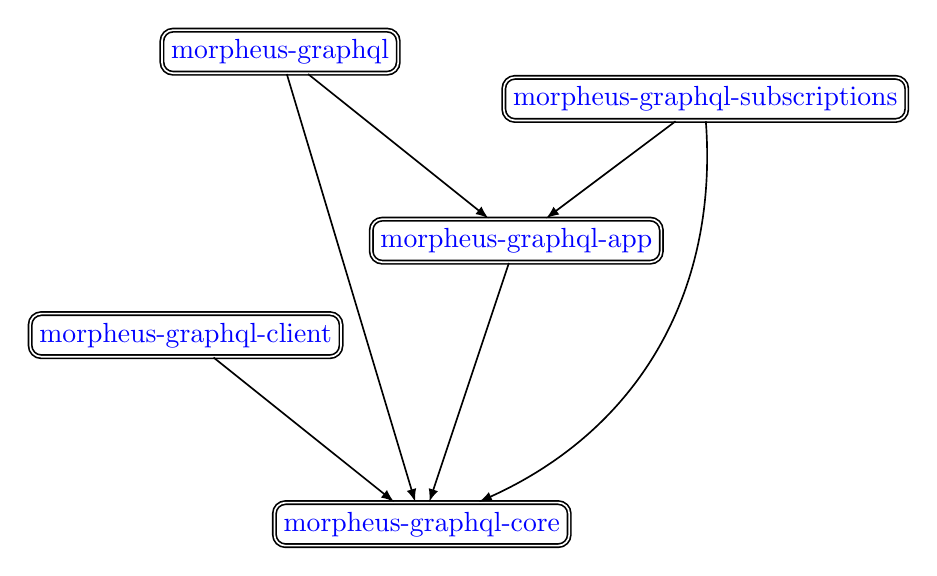
\begin{tikzpicture}[
        scale=.6,
        auto=left,
        -latex ,
        auto ,
        node distance =2 cm and 2cm ,
        % on grid ,
        semithick ,
        package/.style ={ fill=red!20,draw,double,rounded corners ,top color =white ,draw , text=blue , minimum width =1 cm},
    ] 
    \node[package] (core) at (10,0) {morpheus-graphql-core};
    \node[package] (client) at (5,4)  {morpheus-graphql-client};
    \node[package] (app) at (12,6)  {morpheus-graphql-app};
    \node[package] (server) at (7,10)  {morpheus-graphql};
    \node[package] (subs) at (16,9) {morpheus-graphql-subscriptions};
  
    \path (client) edge (core);
    \path (app)  edge (core);
    \path (server)  edge  (core);
    \path (server)  edge  (app);
    \path (subs)  edge  (app);
    \path 
        (subs) 
            edge [bend left =35] 
        (core);  

\end{tikzpicture}
\end{center}
\end{figure}

\end{frame}

%!TEX root = ../../main.tex



\section{Mapping Rules}

\begin{frame}\frametitle{Mapping Rules}

% The underlying entity of every GraphQL schema is a type. 
% Thereby there are six types of named type definitions 
% (Scalar, Object, Interface, Union, Enum, Input) 
% and two wrapping types (List, Non-Null)~\cite{gql-spec}. 
\footnotesize
\begin{itemize}

  \li{Positional Constructors} GraphQL fields must always have names~\cite{gql-spec}. 
  That why we assume that a constructor without field selectors is enumerated like an array.
  
  \importHS{positional-cons}{Positional Constructors}

  \li{Unit Type} The unit type indicates the absence of a specific value and serves as a placeholder when no other value exists or is needed~\cite{fsharp-unit}. GraphQL does not provide it~\cite{gql-spec}. 

  \importGQL{unit-type}{GraphQL Unit Type Definition}

\end{itemize}
\end{frame}

\subsection{Wrapping Types}
\begin{frame}\frametitle{Wrapping Types}

GraphQL defines two primitive wrapping types: List and Non-Null~\cite{gql-spec}.

\begin{itemize}

  \li{Non-Null} GraphQL types are nullable by default: e.g., a scalar string can return either zero or a string value. The non-null type wraps another type and means that the resulting value will never be null~\cite{gql-spec}.

    type \expr{Maybe Int} for nullable GraphQL type \expr{Int} and type \expr{Int} for the non-null GraphQL type \expr{Int!}

  \li{List} GraphQL List is a collection of homogeneous elements, where the elements are ordered and serialized according to their type~\cite{gql-spec}. 
\end{itemize}

\end{frame}

\subsection{Scalars}
\begin{frame}\frametitle{Scalars}

Scalar types represent primitive leaf values in a GraphQL type system. They can be represented as strings. GraphQL offers built-in scalar and enables users to extend the type system with additional scalars with their semantic meaning~\cite{gql-spec}.

Since scalar types have no structural representation, we will impose no restriction and allow any type to represent a scalar type if it has appropriate parse and serialization methods.

\begin{itemize}

  \item Int: Int
  %  This scalar type represents a signed numeric 
    32-bit non-fractional value~\cite{gql-spec}. 

  \item Float: Double
  %  GraphQL-Float represents signed fractions with double precision~\cite{gql-spec}

  \item String: Text
  %  GraphQL String is a regular UTF-8 string for text data~\cite{gql-spec}. Haskell represents strings through the built-in list type. It allows the programmer to use the polymorphic list combinations for complex string manipulations.
  % However, it is also extremely inefficient. An alternative to String is the type Text, which is an array-based string representation that is faster and more compact than String~\cite{string-vs-text,string-types-alexeyshmalko,string-types-fpcomplete,hackage-data-text}. 
  \item Boolean: Bool
  % Since this represents typical Boolean values (true and false)~\cite{gql-spec}, it is represented as a type Bool.
  \item ID:  defined custom data type ID 
  % is a unique identifier that should always be serialized as a String (although it is often numeric)~\cite{gql-spec}. Accordingly, we declare a new data type ID with parse and serialization implementations that meet this specification.
\end{itemize}

\end{frame}

\subsection{Enums}

\begin{frame}\frametitle{Enums}

enum types describe the set of possible independent, unique values~\cite{gql-spec}. They correspond to the algebraic data type with empty fields. The type is only represented as an enum if all its constructors are empty.

\importHS{enum}{GraphQL Enum}
\importGQL{enum}{GraphQL Enum}

\end{frame}

\subsection{Input Object And Field Arguments}
\begin{frame}\frametitle{Input Object And Field Arguments}

A GraphQL input objects and arguments are is a sets of labeled input values~\cite{gql-spec}. They resemble single constructor Haskell records. 

\importHS{input-object}{GraphQL Input Object in Haskell}
\importGQL{input-object}{Input Object Deity}

\subsection{Objects}

\end{frame}

\begin{frame}\frametitle{Objects}

% \subsection{Interfaces}
% \label{sec:mapping:interfaces}

% As in object, interfaces represent a list of named fields and their arguments. Therefore the same rules apply to their fields as to object fields. Apart from their similarities, there are two main differences. First, an object can implement interfaces, which requires that the object type defines all fields defined by these interfaces. Second, an interface cannot implement another interface~\cite{gql-spec}.

% Haskell has no features like GraphQL interfaces. We can consider type classes as GraphQL interfaces, but they cannot be derived with generics, and we cannot cast them for additional fields in the GraphQL query. Accordingly, our current approach only simulates them and derives them like objects.

GraphQL objects are a set of named fields, where fields themselves consist of argument and return type~\cite{gql-spec}. Hence before we try to define an object, we will define its components.

Object field arguments are a set of all possible argument names with corresponding input types~\cite{gql-spec}. Since they are structurally no different from input objects, we can also represent them with Haskell records. 

% Object fields are functions which occasionally accept arguments and return corresponding values. An object field without an argument (e.g. \expr{field: Int}) is equivalent to a function with empty arguments (e.g. \expr{field(): Int})~\cite{gql-spec}.
% Accordingly, we represent Haskell functions as object fields with arguments and leftovers as fields without arguments. 

We represent the object types with records. Furthermore, they get the type parameter \expr{m} for modularity.
This technique allows types to be defined independently of the resolver operations, and the concrete operations can be passed recursively from parent to child. 

\importHS{object-type}{GraphQL Object in Haskell}
\importGQL{object-type}{}

\end{frame}

\subsection{Unions}
\begin{frame}\frametitle{Unions}

GraphQL unions represent an object, one of the possible alternative object types, but do not provide guaranteed fields between them~\cite{gql-spec}. This definition is very similar to the definition of algebraic data types, but Haskell presents it in different ways. While in GraphQL, we only refer to the object type in the list of possible types, in Haskell, we put each of them into a specific constructor. Furthermore, in Haskell, we can create alternative objects only with constructors without defining their types.

% we can generate GraphQL object types \expr{Cat} and \expr{Dog} for the two constructors of the data type \expr{Animal} and build a GraphQL union type from them. However, it raises difficulties if some member type is already defined.

% \importHS{morpheus/code}{union}{Mapping GraphQL Union}

% Let us assume one may want to define a union type animal with variants dog and cat, where the type dog is already defined. 
% \refHS{union-mixed} defines the variant dog with a single field positional constructor and the variant cat with a record constructor.
% However, we get the union type with packed variants \expr{UnionDog | Cat} instead of the expected \expr{Dog | Cat}. The approach creates a new object type \expr{UnionDog} for the variant dog instead of referencing it directly. So we must someway unpack type \expr{Dog} from it.

% \importHS{morpheus/code}{union-mixed}{Mapping GraphQL Union}

\importHS{union-unpack}{Union Types}
\importGQL{union-unpack}{Union Types}

% On the one hand, we could unpack single field constructors where a field type is an object, but that does not work because the constructor \expr{Cat} also has a single field \expr{name} with the object type \expr{Name}.  On the other hand, we could unpack single-field constructors with a name prefixed with "Unpack," but that would allow multiple unpacking of the same type in a single union. Therefore, we unpack constructors, where the name is the concatenation of the type constructor name and the referencing type name. That way, the compiler in \refHS{union-unpack} unpacks the type \expr{Dog} but generates a new object type \expr{Cat}.

% So far, we have only covered alternatives 
% with at least one field, but we also have 
% to deal with empty variants. 
% For example, one might want to add support 
% cases of unidentified animals without having 
% information about these species \seeHS{union-empty-cons}. 
% The current derivation approach presents 
% empty constructors as empty object definitions, 
% but GraphQL does not support empty object 
% definitions~\cite{gql-spec}. 
% To represent them as valid object definitions, 
% we can assign them a field \expr{\_} with the 
% type \expr{Unit}, which indicates that 
% the field does not contain any information 
% and reduces confusion . 
% As a result, \refHS{union-empty-cons} generates the schema defined in \refGQL{union-empty-cons}. As we can see, the GraphQL object \expr{Cat} represents the constructor \expr{Cat}, and the GraphQL object \expr{Unidentified} with only the field \expr{\_} represents the empty constructor \expr{Unidentified}. 

\end{frame}

\begin{frame}\frametitle{Determining GraphQL Types in Haskell}
\subsection{Determining GraphQL Types in Haskell}

So far, we have only covered the mapping of GraphQL types to corresponding Haskell types. However, we have not yet addressed how the approach decides which GraphQL type to derive from the Haskell data type.  This section presents the following rules that the compiler applies for a given execution order to achieve deterministic derivation.

\begin{enumerate}
  \li{Scalar, Wrapper, Interface} The structure of these types does not provide sufficient information to determine their kinds.Therefore they must explicitly provide associated kinds that determine their GraphQL type representation. The remaining types can be automatically derived based on their data type structure and place of use.
  
  \li{Field Arguments} Derive field arguments if the type is used as an argument of the object field. 

  \li{Enum} Derive enum if all data type constructors are empty.

  \li{Object} Derive object if the type has a single non-empty constructor, and its parent \footnote{Type A is the parent type of type B if it has a field that refers to type B} is Object or Union. 
  
  \li{InputObject} Derive input object if the type has a single non-empty constructor, and its parent is InputObject or Field Arguments.

  \li{Union} Derive Union if the type has multiple constructors and its parent is Object or Union.

  \li{Fail} All other types are not supported. The compiler will fail at this point. Note: The real implementation also supports the case of deriving input unions. However, since GraphQL does not support them, they are not mentioned in this work.

\end{enumerate}

\end{frame}


\section{Schema Derivation} 
\begin{frame}\frametitle{Schema Derivation}

GraphQL models the schema as a graph, where nodes are types (objects), and the type consists of fields. These fields have a name and a reference to another type (edges). Technically, the graph starts with a root node that branches to query subscription and mutation nodes and then to API-specific types~\cite{migrating-to-gql}. Accordingly, the deep-first search, starting from the root node, can derive all schema types. Therefore, we have decided to derive the schema only from the root type. However, the simple application of deep-first search leads to a loop if the graph has cycles (in our case, if the type refers directly or indirectly to itself). Therefore we use the deep-first search with cycle checking.

% The cycle check requires a unique key for the identification of each node. 
% Since two types in different modules can have the same name, we cannot use the type name as the key. However, the type fingerprint provided by the module \axpr{Typeable} is the right candidate for it.    
% Additionally, one type can derive input and output types. 
% So we do not want to skip generating the input type if the output type was already generated for the same type since they are not the same for the GraphQL type system.
% Therefore, we use the product \expr{(Context, Fingerprint)} as the key for each node, where \expr{Context} can be one of the following values: \expr{Input}, \expr{Output}. 
% As a result, we can define the function \expr{deriveSchema}\srcGithub{src/Data/Morpheus/Server/Deriving/Schema.hs}, which receives the root type and derives a schema from it. \refHS{derive-schema} presents the signature of this function.

\end{frame}

%!TEX root = ../main.tex
\section{Examples}

\begin{frame}\frametitle{Morpheus}

repository: \url{https://github.com/nalchevanidze/morpheus-haxl-example}

\end{frame}
\section{Evaluation}

\begin{frame}[allowframebreaks]\frametitle{Evaluation}

\begin{block}{Maintainability}

  \begin{itemize}
  
    \li{Low Boilerplate and Familiarity} The library follows a code-first approach and and derives api from native Haskell types based on data-type-generic programming. the approach is familiar reduces boilerplate and improves maintainability.

    \li{Modularity}
      The library architecture divides functionalities into separate, coherent packages. 
    
      The modularity of the API definition is achieved by introducing parameterized resolver types. They decouple the types from the accessible operations, and thus one can use one data type for different operations.

  \end{itemize}

\end{block}


\begin{block}{Reliability}

\begin{itemize}

  \li{Type Safety} 
    \begin{enumerate}

      \li{Deterministic deriving} The mapping rules cover all Haskell algebraic data types.

      \li{Resolver validity} The Haskell compiler reports any value mismatch at compile time.
      
      \li{Schema validity} Haskell and GraphQL adopt different types of type systems. That why the Haskell compiler cannot check the validity of all GraphQL-specific rules. Therefore, to ensure schema validity, we provide the function \expr{compileTimeSchemaValidation}, which takes the \expr{RootResolver} type signature and fails if the schema is invalid.
    
    \end{enumerate}

  \li{Complience with GraphQL Specifications} The library meets all the critical parts of the specifications. However, there are also small deviations in favor of flexibility, e.g., the use of \expr{Int} instead of \expr{Int32}. Moreover, interfaces and directives are still not fully implemented. 

\end{itemize}

\end{block}

\begin{block}{Efficiency} we used the type \expr{Text} instead of \expr{String}. the library only executes the resolvers necessary for the query. The library is extensible with Haxl, which allows efficient reuse of resolvers without running into the n+1 selects problem.

\end{block}

\end{frame}

\begin{frame}\frametitle{General Overview}

Our prototype meets our predefined requirements, with an acceptable tradeoff between flexibility and compliance. We provide a straightforward approach to GraphQL API definitions while still guaranteeing type safety. Besides, users can achieve efficiency in the combination of Morpheus GraphQL and Haxl, as GraphQL solves over-fetching and under-fetching problems for a client and  Haxl for the backend.

Nevertheless, we run into some limitations: First, Haskell permits different naming of values and types than GraphQL. Second, sets and non-empty collections cannot be modeled in GraphQL because it provides only list types for collections. Therefore, sets and non-empty collections are represented to GraphQL clients with regular lists, and the client cannot check the validity of input values at compile time. Third, since Haskell makes no distinction between input and output types, mapping Haskell types requires support for input unions, which is not supported by GraphQL. Fourth, Haskell does not provide interfaces, so we do not yet have a satisfying way to support them. 
\end{frame}

\section{Conclusions}

\begin{frame}\frametitle{Advantages}

The presented approach successfully implements the requirements and provides:

\begin{itemize}
    \item easy-to-use interface while ensuring type safety.
    \item We preferred intuitive design over extensibility.
    \item The library can be learned quickly by beginners.
    \item Importing schemas from SDL facilitates quick starts and migration from other languages.
    \item A type-safe client package allows developers to implement entire applications in one language or even query data for resolvers from other GraphQL servers.
    \item \expr{Apps} are members of the type class semigroup and can be composed.
\end{itemize}

\end{frame}

\begin{frame}\frametitle{Limitations}

\begin{itemize}
    \item Haskell permits different naming of values and types than GraphQL. 
    \item sets and non-empty collections cannot be modeled in GraphQL because it provides only list types for collections. 
    \item mapping Haskell types requires support for input unions, which is not supported by GraphQL. 
    \item Haskell does not provide interfaces, so we do not yet have a satisfying way to support them. 
\end{itemize}

\end{frame}

\begin{frame}\frametitle{Outlook}

\begin{itemize}
    \li{Support Interfaces} representation of interfaces with "type guards" on unions. 
    \li{Type-Level Curried Arguments} flexible argument definitions for a small number of arguments than our current approach since the user does not have to define a new data type for each field. 
    \li{Custom Collections} Since GraphQL has only one type (List) for collections, we cannot represent collections with certain constraints. 
    \li{Support Directives}Since the GraphQL specification does not specify a particular implementation strategy for directives, it is up to each server library to provide a suitable API~\cite{schema-directives}.
    \li{Support Input Unions} GraphQL does not support input unions. While this function's value is essentially understood, its implementation is not cleared~\cite{gql-spec-input-unions}. 

\end{itemize}

\end{frame}

\setLayout{blank}
%!TEX root = ../../main.tex

\section*{Thanks}
\setBGColor{white}
\begin{frame}
    
    \centering
    \vspace{2cm}
    
    \textbf{\Huge Danke!}
 
    \ \\
    \ \\
    \textbf{Fragen oder Anregungen?}
    
    \text{\footnotesize d.nalchevanidze@gmail.com}
    
    \vspace{1.5cm}
    \begin{figure}
        \centering
        \begin{subfigure}{0.2\textwidth}
            \centering\pgfuseimage{logo_title}
        \end{subfigure}%      
    \end{figure}
\end{frame}
\setLayout{titlepage}
\titlepage
\setLayout{regular} 

\nocite{*}
\begin{frame}[plain, noframenumbering,allowframebreaks]{References}
    \printbibliography
\end{frame}

\end{document}